% !TeX spellcheck = de_CH
\documentclass[11pt,a4paper,english,oneside]{book}

\usepackage{etex} %Because of many packages --> Extended TeX.
\usepackage[left=1in, right=1in]{geometry} %Helps to structure the paper layout.
\usepackage[Lenny]{fncychap} %Design of the thesis.
\usepackage[utf8]{inputenc} %Due to vowels.
\usepackage[T1]{fontenc}
\usepackage[ngerman]{babel} %Define the language style.

% german language for appendix header
\addto\captionsngerman{\let\appendixtocname\appendixname%
\let\appendixpagename\appendixname}

\usepackage{dsfont} %Nice style for the indicator function.
\usepackage{fancyhdr} %To customize the headers and footers.
\usepackage{booktabs} %In case you need \cmidrule or \addlinespace in tables.
\usepackage[hang,bottom,stable,multiple]{footmisc} %Style of footnotes.
\usepackage{appendix} %For the \appendixpage command.
%Load some mathematical packages.
\usepackage{amsmath}
\usepackage{amsfonts}
\usepackage{amsmath}
\usepackage{amssymb}
\usepackage{mathtools}
\usepackage[sort,round]{natbib} %For the bibliography.
\usepackage{etoolbox} %To remove the page number on \appendixpage.
\usepackage{amsthm} %For theorems, definitions etc.
\usepackage{thmtools} %For theorems, definitions etc.
\usepackage{setspace} %Use double spacing.
\usepackage{lipsum} %For the \lipsum command to generate a text.
\usepackage{datetime} %For the specification of the date.
%\usepackage{tocloft} %The ToC, LoF and LoT each appear not necessarily on a new page.
\usepackage{graphicx,listings,xcolor,textcomp} %For the graphics, listings etc.
\usepackage{mcode} %To implement a Matlab code.
\usepackage[margin=10pt, font=small, labelfont=bf, labelsep=endash]{caption} %Customize the captions.
\usepackage{chngcntr} %To use counterwithout.
\usepackage{epstopdf} %For inserting .eps files into the document.
\usepackage{hyperref} %Must be loaded at the end.
\usepackage{xparse} %Load for \NewDocumentCommand command.
\usepackage{cleveref} %For the command \cref, load after hyperref.
\usepackage{arydshln} %Due to the capability to draw horizontal/vertical dash-lines.
\usepackage{array,hhline} %To create tables and matrices.
\usepackage{rotating} %To rotate a table.
\usepackage{tabularx} %An extended version of tabular.

%Setup of the reference links.
\hypersetup{
     colorlinks=false,
     linkcolor=blue,
     citecolor=blue,
     filecolor=magenta,
     urlcolor=blue}

%Define some reasonable margins.
\setlength{\textwidth}{6.6in}
\setlength{\textheight}{8.8in}
\setlength{\topmargin}{-0.1in}
\setlength{\oddsidemargin}{0in}
\setlength{\parskip}{1mm}

\bibliographystyle{abbrvnat} %Reference style.
\allowdisplaybreaks[1] %Page breaks of equations are allowed, but avoided if possible. 2-4 more relaxed.

%New command for the UZH logo.
\newcommand*{\plogo}{
\includegraphics{logo_hsr.pdf}}

%New command for the differential d to have an ordinary d.
\makeatletter
  \newcommand{\ud}{\mathrm{d}}
\makeatother

%Remove page number on \appendixpage. Use the package 'etoolbox'.
\makeatletter
\patchcmd{\@chap@pppage}{\thispagestyle{plain}}{\thispagestyle{empty}}{}{}
\makeatother

%Declare Definitions, Theorems etc.
%%%%%%%%%%%%%%%%%%%%%%%%%%%%%%%%%%%%%%%%%%%%%%%%%%%%%%%%%%%%%%%%%%%%%%%%%%%%%%%%%%%%%%%%%%%%%%%%%%%%%%%%%%%%%%%%%%%
\declaretheorem[style=definition,qed=$\blacktriangleleft$, numberwithin=chapter]{remark} %additional options; numberwithin=,..., see 'Thmtools' Users’ Guide
\declaretheorem[style=definition,qed=$\triangle$,numberwithin=chapter]{definition}
\newtheorem{ass}{Assumption}[chapter]
\newtheorem{prop}{Proposition}[chapter]
\newtheorem{lemma}{Lemma}[chapter]
\declaretheorem[style=definition,qed=$\perp$,numberwithin=chapter]{example}
\newtheorem{theorem}{Theorem}[chapter]
\newtheorem{coroll}{Corollary}[chapter]
%%%%%%%%%%%%%%%%%%%%%%%%%%%%%%%%%%%%%%%%%%%%%%%%%%%%%%%%%%%%%%%%%%%%%%%%%%%%%%%%%%%%%%%%%%%%%%%%%%%%%%%%%%%%%%%%%%%

%Readjust the numbering.
\counterwithout{footnote}{chapter}
\numberwithin{equation}{chapter}

%\setlength{\parindent}{0cm} %Uncomment this if you don't want to have indents.

%----------------------------------------------------------------------------------------
%	TITLE PAGE
%----------------------------------------------------------------------------------------
\newcommand*{\titleGP}{\begingroup %Create the command for including the title page in the document.
\centering %Center all text.
\vspace*{\baselineskip} %White space at the top of the page.
\plogo\\[2\baselineskip] %University Logo.
\rule{\textwidth}{1.6pt}\vspace*{-\baselineskip}\vspace*{2pt} %Thick horizontal line.
\rule{\textwidth}{0.4pt}\\[\baselineskip] %Thin horizontal line.
{\LARGE [ Graphs-Visualization-Service ]}\\[0.2\baselineskip] %Title.
\rule{\textwidth}{0.4pt}\vspace*{-\baselineskip}\vspace{3.2pt} %Thin horizontal line.
\rule{\textwidth}{1.6pt}\\[2\baselineskip] %Thick horizontal line.
\scshape %Small caps.
Studienarbeit \\[2\baselineskip]
Eingereicht zur Teilerfüllung der Voraussetzungen für den Bachelor of Science in Informatik an der HSR \par
\vspace*{2\baselineskip}


Autoren\\
{\Large [ Michael Wieland ] \\ [5pt]}
mwieland@hsr.ch \\

{\Large [ Murièle Trentini ] \\ [5pt]}
mtrentin@hsr.ch \\

\vspace*{2\baselineskip}
Betreuer\\
{\Large [ Thomas Letsch ] \\[5pt]
\small Dozent für Informatik an der \\[5pt]Hochschule für Technik Rapperswil\par}
\vspace*{2\baselineskip}

Auditor\\
{\Large [ Name ] \\[5pt]}
\vspace*{2\baselineskip}

\vfill
{\scshape Zeitraum: 18.09.2017 - 15.12.2017} \\[0.3\baselineskip]
\endgroup}


%Special header and footer style for the executive summary and Task Assignment section.
\fancypagestyle{firststyle}{%
  \fancyhf{}%
  \renewcommand{\headrulewidth}{0pt}
  \fancyfoot[C]{\thepage}}

%Customize headers and footers.
\pagestyle{fancy}
\fancyhead[R]{\thepage}
\fancyhead[L]{\rightmark}
\fancyfoot[L]{[ Murièle Trentini | Michael Wieland ]}
\fancyfoot[C]{}
\fancyfoot[R]{[ GVS ]}

%Define the signature line with dots.
\NewDocumentCommand \dotbox {o O{.5\linewidth} m O{3ex} O{\linewidth}}
{
  \begin{minipage}{7cm}
    \makebox[7cm][l]{\,.\dotfill}
    \\
    \makebox[7cm][l]{\,#3}
  \end{minipage}
}

\begin{document}
\thispagestyle{empty}
\titleGP
\newpage
\doublespacing
\setcounter{page}{1}
\pagenumbering{Roman}
\section*{Abstract}
\thispagestyle{firststyle}


\newpage

\section*{Management Summary}
\thispagestyle{firststyle}

\subsection*{Motivation}

\subsection*{Ziele}

\subsection*{Ergebnisse}

\subsection*{Ausblick}

\tableofcontents
\listoffigures
\listoftables
\newpage
\pagenumbering{arabic}
% \part{[ Part title ]}
\chapter{[ Anforderungsanalyse ]}

\section{[ Ausgangslage ]}

\section{[ Mehrwert ]}

\section{[ Aufgabenstellung ]}

\section{[ User Stories ]}

\section{[ Use Cases ]}

\subsection{Brief}

\subsection{Fully Dressed}

\section{[ Domainanalyse ]}



%\part{ [ Realisierung ] }

\chapter{ [ Realisierung ]}

\section{ [ Architektur ] }

\section{ [ UI Design ] }

\subsection{Konzept}

\subsection{Icons}

\subsection{Farben}

\subsection{Wireframes}

\section{ [ Testing ] }


\chapter{ [ Projektmanagement ]}

\section{ [ Projektorganisation ] }

\section{ [ Meilensteine ] }

\section{ [ Zeitmanagement ] }

\section{ [ Risikomanagement ] }


\chapter{ [ Examples ]}

\section{[ Section Title ]}

[...] Between sections and subsections, you may want to add at least three or four sentences (or more), instead of leaving it blank.

\subsection{[ Subsection Title ]}

[...] In the next subsection, there is some sample text with figures and tables. [...]




\subsection{Pricing Errors}


[...] we present the root mean squared pricing errors (RMSEs) and the mean pricing errors (MPEs) on caps and swaptions implied volatilities, defined as the difference in percentage points between the model-implied values and the market-implied volatility quotes. Overall, we find that, for intermediate and long maturities, our model performs remarkably well. The cap pricing errors in Table \ref{Table2} indicate that the model's performance suffers mostly at the short end of option maturities, especially for the one-year maturity. Short maturity contracts are underpriced by the model. However, the pricing performance considerably improves with increasing maturity. For longer maturities, a tendency exists to underprice out-of-the money and overprice in-the-money contracts.



\begin{table}[htbp!]
	%\renewcommand{\arraystretch}{1.10}
	%\centering
	\caption[Pricing Errors for the Caps Market]{ Pricing errors for the caps market. \label{Table2} \newline
		Reported are sample averages of the root mean squared errors (RMSEs) and mean pricing
		errors (MPEs) for caps implied volatilities, defined as the difference in percentage points between the model-implied values and the market-implied volatility quotes.
		Each row represents one cap maturity, and columns represent the moneyness of the cap.}
	\setlength{\tabcolsep}{6pt}
	\vspace{0.2cm}
	%\begin{center}
	\begin{tabular}{@{}lcrrrrrrrrrrrr@{}}
		\toprule & \multicolumn{5}{c}{RMSE}
		&& \multicolumn{5}{c}{MPE} \\
		\cmidrule(r){2-6}  \cmidrule(r){8-12}
		{Maturity}  & 0.80 & 0.90 & 1.00 & 1.10 & 1.20 && 0.80 & 0.90 & 1.00 & 1.10 & 1.20 \\
		\midrule
		%\multicolumn{2}{l}{A: Root mean squared error} & & &  & & & \\
		One year  & 16.86   &   18.62   &   20.15   &  20.30   &  22.03 & &  -10.73  & -11.08  & -11.95   &-12.32  &-15.96      \\
		Two years  & 12.26   &   11.71   &    9.79   &   9.57   &   9.85 & &   -8.64  &  -8.77  &  -6.99   & -6.17  & -7.01      \\
		Three years  &  8.78   &    6.75   &    4.75   &   4.19   &   4.02 & &   -6.67  &  -5.15  &  -3.44   & -2.52  & -2.59      \\
		Four years  &  6.47   &    4.29   &    2.25   &   1.66   &   2.03 & &   -4.81  &  -2.98  &  -1.40   & -0.48  & -0.06      \\
		Five years  &  4.98   &    2.94   &    1.35   &   1.26   &   2.18 & &   -3.41  &  -1.67  &  -0.30   &  0.56  &  1.29       \\
		Six years  &  4.28   &    2.36   &    1.41   &   1.68   &   2.50 & &   -2.63  &  -0.92  &   0.31   &  1.11  &  1.97      \\
		Seven years  &  3.91   &    2.16   &    1.71   &   2.08   &   2.71 & &   -2.07  &  -0.38  &   0.74   &  1.48  &  2.25      \\
		Eight years  &  3.63   &    2.07   &    1.89   &   2.27   &   2.80 & &   -1.71  &  -0.07  &   0.95   &  1.63  &  2.33      \\
		Nine years  &  3.48   &    2.09   &    2.04   &   2.42   &   2.88 & &   -1.35  &   0.20  &   1.15   &  1.79  &  2.41      \\
		Ten years &  3.37   &    2.15   &    2.18   &   2.54   &   2.95 & &   -1.06  &   0.42  &   1.31   &  1.91  &  2.47      \\
		\bottomrule
	\end{tabular}\\
	%\vspace{0.5pt} \\
	%\end{center}
\end{table}
%\end{center}



For the ATM swaptions implied volatilities in Table \ref{Table3}, we observe a similar pattern. The model struggles mostly for short option maturities and short swaption tenors, an observation that also holds true for the non-ATM swaptions. However, across moneyness no clear pattern emerges in terms of over- and underpricing as is the case for in-the-money and out-of-the-money caps.



\begin{sidewaystable}[htbp!]
	%\begin{table}[htbp!]
	%\renewcommand{\arraystretch}{1.10},
	%\centering
	\caption[Pricing Errors for ATM Swaptions]{ Pricing errors for at-the-money (ATM) swaptions. \newline
		Reported are sample averages of the root mean squared errors (RMSEs) and mean pricing
		errors (MPEs) for ATM swaptions implied volatilities, defined as the difference in percentage points between the model-implied values and the market-implied volatility quotes. Each row represents one swaption maturity, and each column represents one swap tenor.}
	\label{Table3}
	\vspace{0.2cm}
	\setlength{\tabcolsep}{6pt}
	%\begin{center}
	\begin{tabular}{lrrrrrrrlrrrrrrr}
		\toprule &
		\multicolumn{7}{c}{RMSE} &&
		\multicolumn{7}{c}{MPE} \\
		\cmidrule(l){2-9}  \cmidrule(l){10-16}
		& \multicolumn{7}{c}{Swap tenor} &&
		\multicolumn{7}{c}{Swap tenor} \\
		\cmidrule(l){2-9}  \cmidrule(l){10-16}
		\multicolumn{1}{l}{{Option}} & \multicolumn{1}{l}{One} & \multicolumn{1}{l}{Two} & \multicolumn{1}{l}{Three} & \multicolumn{1}{l}{Four} &
		\multicolumn{1}{l}{Five} & \multicolumn{1}{l}{Seven} & \multicolumn{1}{l}{Ten} & & \multicolumn{1}{l}{One} &  \multicolumn{1}{l}{Two} & \multicolumn{1}{l}{Three} & \multicolumn{1}{l}{Four} & \multicolumn{1}{l}{Five} & \multicolumn{1}{l}{Seven} & \multicolumn{1}{l}{Ten} \\
		
		\multicolumn{1}{l}{maturity} & \multicolumn{1}{l}{year} & \multicolumn{1}{l}{years} & \multicolumn{1}{l}{years} & \multicolumn{1}{l}{years} &
		\multicolumn{1}{l}{years} & \multicolumn{1}{l}{years} & \multicolumn{1}{l}{years} & & \multicolumn{1}{l}{year} &  \multicolumn{1}{l}{years} & \multicolumn{1}{l}{years} & \multicolumn{1}{l}{years} & \multicolumn{1}{l}{years} & \multicolumn{1}{l}{years} & \multicolumn{1}{l}{years} \\
		
		
		\midrule
		%\multicolumn{3}{l}{A: Root mean squared error} &  \\
		Three months	&	21.16  & 9.66  &  4.46 & 4.82  & 5.94&8.30  & 10.32 && -14.13  & -7.24&  -1.97&  0.72 &   1.77&  5.09&   7.38\\
		Six months	&	19.53  & 7.93  &  2.58 & 2.60  & 3.78&6.17  &  7.89 && -13.67  & -6.05&  -1.45&  0.90 &   1.93&  4.35&   6.10\\
		One year	&	12.72  & 5.27  &  1.74 & 1.52  & 2.27&3.82  &  4.95 && -8.81   &-3.21 & -0.43 &  0.86 &  1.48 & 2.83 &  3.84\\
		Two years	&	 4.20  & 2.20  &  1.49 & 1.31  & 1.36&1.61  &  2.04 && -1.03   & 0.15 &  0.61 &  0.71 &  0.65 & 0.75 &  1.13\\
		Three years	&	 2.34  & 1.75  &  1.38 & 1.18  & 1.13&1.22  &  1.41 &&  1.33   & 1.16 &  0.86 &  0.51 &  0.16 &-0.05 & -0.03\\
		Four years	&	 2.36  & 1.65  &  1.29 & 1.08  & 1.19&1.25  &  1.40 &&  1.85   & 1.20 &  0.71 &  0.14 & -0.17 &-0.53 & -0.65\\
		Five years	&	 2.36  & 1.65  &  1.35 & 1.25  & 1.32&1.51  &  1.67 &&  1.89   & 1.13 &  0.49 & -0.07 & -0.47 &-0.73 & -0.88\\
		Seven years	&	 2.10  & 1.53  &  1.36 & 1.32  & 1.32&1.54  &  1.80	&&  1.44   & 0.73 &  0.28 & -0.16 & -0.44 &-0.74 & -1.07\\
		Ten years   &  1.93   & 1.56  &  1.40 & 1.39  & 1.42&1.53  &  1.72 &&  1.32   &0.88  &  0.50 &  0.22 & -0.01 & -0.47& -0.76\\ \bottomrule
	\end{tabular}\\
\end{sidewaystable}



The substantially higher pricing errors for the caps and swaptions market at shorter maturities call for further investigation.
Ultimately, the caps and swaptions markets must be closely connected, as they both originate from derivatives written on the forward LIBOR. However, during periods of extreme market turmoil, the two markets might exhibit different behaviors due to differences in how the uncertainty regarding the intensified liquidity situation in the interbank market propagates through the caps and swaptions markets. Therefore, we next analyze the behavior of the pricing errors across time to see whether the caps and swaptions market become disintegrated or whether they suffer from the same deficiencies.

[ Just added some additional arbitrary text here... ]
% Just remove the command below:
\lipsum



\subsection{A Note on Generating Figures}



In Figure \ref{output2}, we plot the time series of RMSE  (Panel A) and the MPE (Panel B) for caps implied volatilities. We split the time series into long maturities and short maturities. For the first period of our data sample with the financial crisis already in full swing, the pricing errors in terms of RMSE remain remarkably low. In addition, until October 2008, we do not observe a bias in the model's pricing performance with the MPE close to zero. However, the pricing performance deteriorates considerably around April 2009 with substantial underpricing of short maturity contracts. This mispricing remains high until the end of our sample. Interestingly, this period of persistent mispricing of short maturity contracts coincides with the period of high implied volatilities at these maturities. Hence, our model suffers when the volatility term structure is unusually steep.

\begin{figure}[t!]
	\begin{center}
		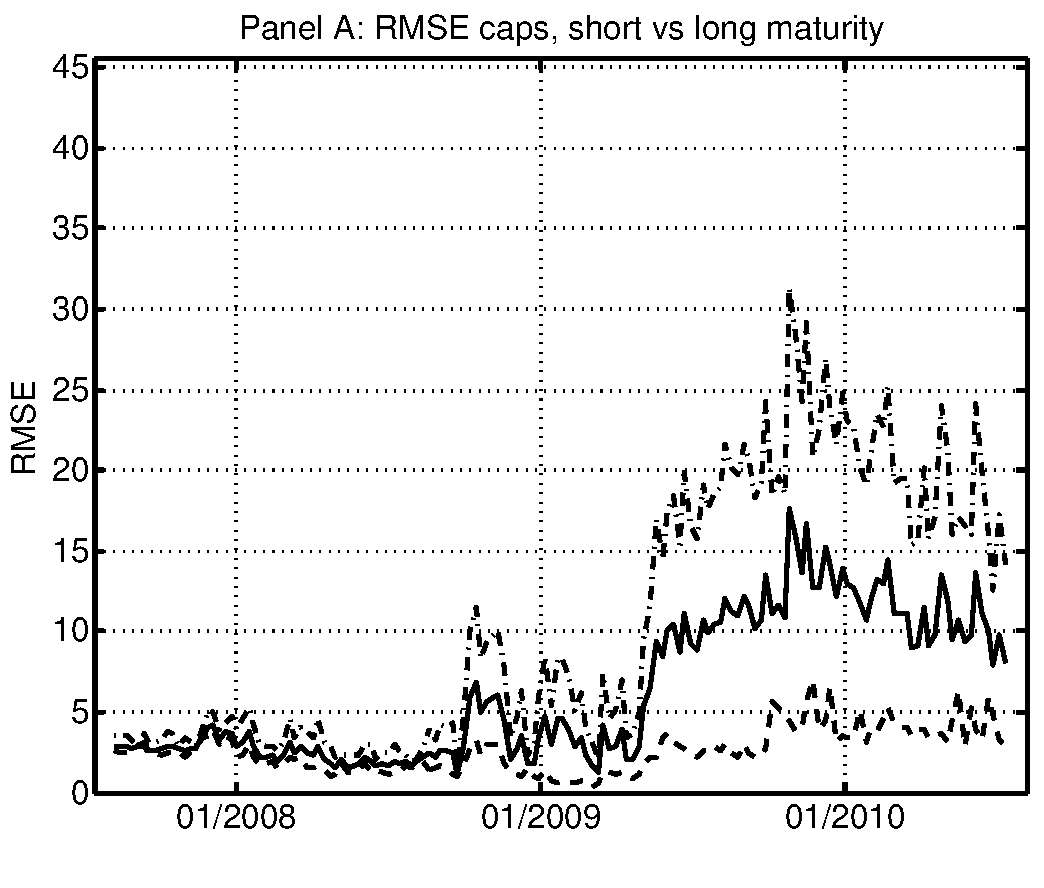
\includegraphics[width=3.20in]{assets/RMSE_ivcapsjoint.pdf}
		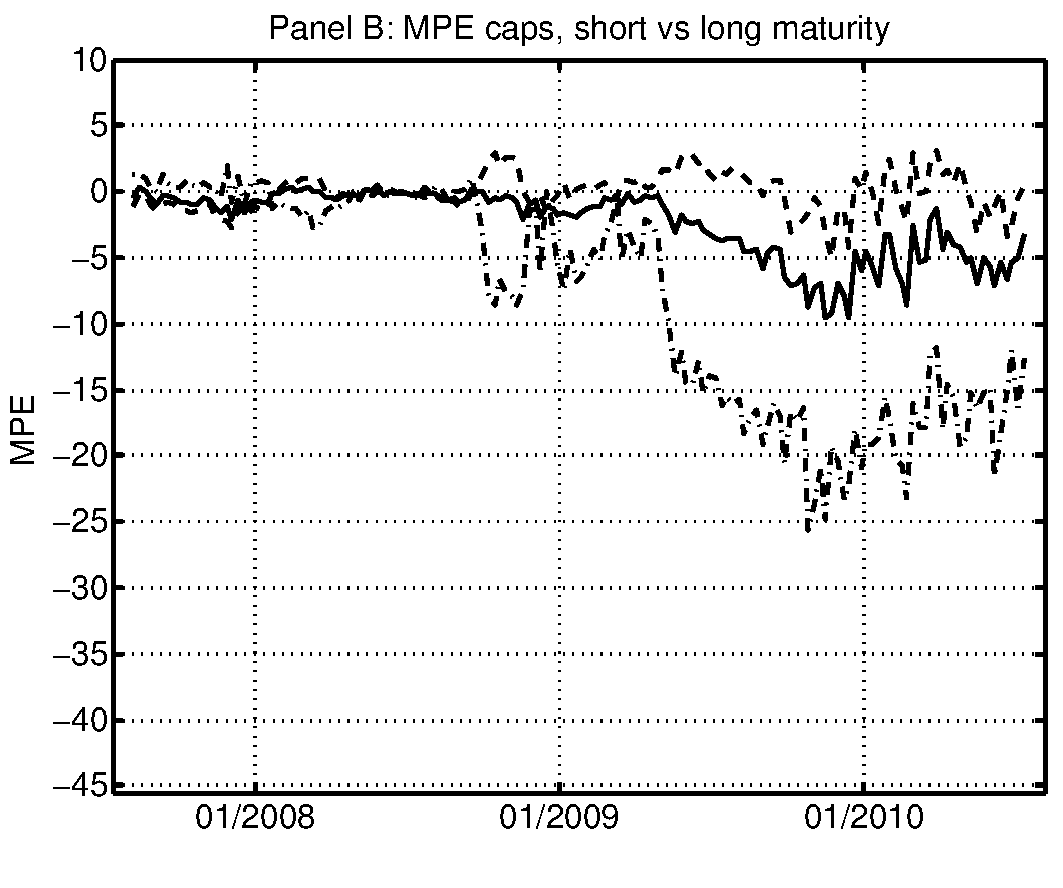
\includegraphics[width=3.20in]{assets/MPE_ivcapsjoint.pdf}
	\end{center}
	\caption[RMSE and  MPE for Caps with Different Maturities]{Root mean squared error (RMSE) and mean pricing error MPE for caps with different option maturities.
		Panels A and B show the RMSE and the MPE in percentage points  across time for caps implied volatilities
		of all maturities (solid line), for maturities up to three years (dash-dotted line), and for maturities of four to ten years (dashed line). Data are
		weekly (Wednesday) spanning our entire data sample August 8, 2007 to
		August 11, 2010; in total, 158 weeks.}
	\label{output2}
\end{figure}


[...] If you use \texttt{PDF} files for input, you should run \texttt{PDFLATEX}. If you use \texttt{EPS} files, then run \LaTeX, then \texttt{DVI}$\rightarrow$\texttt{PS}, then \texttt{PS}$\rightarrow$\texttt{PDF}. To generate \texttt{PDF} files out of \textsc{Matlab}, save them first as \texttt{EPS} files and then use the \texttt{DOS} prompt with the command \texttt{EPSTOPDF}. This gives the nicest results. Also, to generate \textsc{Matlab} graphics in a decent format (lines will not get too thin and the labels will not get too small), use something like this:
\begin{lstlisting}
figure(1)
set(gca,'Box', 'on', 'LineWidth',1.5 ,'FontSize',14)
plot(x,cumprod(1+R(:,2)),x,cumprod(1+R(:,3)),'--',x,cumprod(1+R(:,4)),'-.','LineWidth',1.5)
grid on
datetick('x','mmmyy')
axis([x(1)-10 x(end) 0.5 3.0])
title('Panel A: Equity and commodity indices')
ylabel('Cumulative return')
grid on
legend('MSCI World Total Return', 'MSCI Emerging Market Total Return','DJ UBS Commodity Index')
print('-depsc2', 'cumReturnA.eps' )
\end{lstlisting}

Whatever format you will eventually use, be sure that it looks nice and readable and use it consistently for the whole thesis.


\subsection{A Note on Citations}

[Here are some examples of citations...] Lévy processes cannot capture stochastic volatility, stochastic risk reversal (skewness) and stochastic correlation. These drawbacks can be resolved, at least to some extent, by considering time-changed Lévy processes for which it is possible to generate distributions which vary over time. If the return innovation is modeled by a Brownian motion, we can let the instantaneous variance be stochastic (see, e.g., \cite{SH1993} and \cite{BA1996}) to create dependence of the return increments.\footnote{\cite{CW2004}, for instance, introduced a time-changed Lévy model to capture the leverage effect.}





\newpage

\appendix
\noappendicestocpagenum
\addappheadtotoc
\appendixpage



\renewcommand{\theequation}{A.\arabic{equation}}


\chapter{Proofs}

[ You may also want to add an appendix, if it makes sense. You delegate proofs to the appendix or other material that is essential for the understanding of your work, but would distract the reader if placed in the main text... ]

\section{Proof of Proposition [...] }
[....], we can apply Ito's formula for Lévy processes   to obtain the
dynamics of the forward LIBOR $L(t,T_j)$ to obtain the
dynamics of the forward LIBOR $L(t,T_j)$ under the $T_{j+1}$-forward measure
as follows:
\begin{eqnarray}
\frac{dL(t,T_j)}{L(t,T_j)} &=& b (t,T_{j},T_{j+1}) dt +
\frac{1}{2} \lambda ^2(t,T_j) dt +
\frac{1}{2} V _t^W dt\nonumber \\
&+& \int_{-\infty}^{0}  \left[ e^{x}-1-x \right]
\pi_{J^-}^{\mathbb Q_{j+1}}(dx)\nu _t^J dt + \int_{0}^{\infty} \left[
e^{x}-1-x \right] \pi_{J^+}^{\mathbb Q_{j+1}}(dx)\nu _t^Jdt \nonumber \\
&+& \lambda (t,T_j) dB_{t}^{Q_{j+1}}+ \sqrt{ V _t^W}
dW_{t}^{Q_{j+1}}+ \int_{-\infty}^{0} \left[ e^{ x}-1 \right]
\left[ \mu^- (dt,dx) -
\pi_{J^-}^{Q_{j+1}}(x) dx \nu _t^J dt \right]\nonumber \\
&+& \int_{0}^{\infty} \left[ e^{ x}-1 \right] \left[ \mu ^+ (dt,dx)
- \pi_{J^+}^{Q_{j+1}}(x) dx \nu _t^J dt \right].
\end{eqnarray}
To ensure that $L(t,T_j)$ is a martingale under the
$T_{j+1}$-forward measure, the drift must equal zero, which gives the
drift condition in the proposition. $\blacksquare$



\bibliography{References}

\newpage
\thispagestyle{firststyle}
\section*{Eidesstattliche Erklärung}
Der/Die Verfasser/in erklärt an Eides statt, dass er/sie die vorliegende Arbeit selbständig, ohne fremde Hilfe und ohne Benutzung anderer als die angegebenen Hilfsmittel angefertigt hat. Die aus fremden Quellen (einschliesslich elektronischer Quellen) direkt oder indirekt übernommenen Gedanken sind ausnahmslos als solche kenntlich gemacht. Die Arbeit ist in gleicher oder ähnlicher Form oder auszugsweise im Rahmen einer anderen Prüfung noch nicht vorgelegt worden.\\[2cm]
\dotbox{Ort, Datum} \hfill \dotbox{Unterschrift des/der Verfassers/in}
\hfill \\[2cm]
\dotbox{Ort, Datum} \hfill \dotbox{Unterschrift des/der Verfassers/in}
\end{document}
